\documentclass[12pt,letterpaper,oneside,oldfontcommands]{memoir}
\usepackage{lmodern}
\usepackage{amssymb,amsmath}
\usepackage{ifxetex,ifluatex}
\usepackage{fixltx2e} % provides \textsubscript
\ifnum 0\ifxetex 1\fi\ifluatex 1\fi=0 % if pdftex
  \usepackage[T1]{fontenc}
  \usepackage[utf8]{inputenc}
\else % if luatex or xelatex
  \ifxetex
    \usepackage{mathspec}
  \else
    \usepackage{fontspec}
  \fi
  \defaultfontfeatures{Ligatures=TeX,Scale=MatchLowercase}
\fi
% use upquote if available, for straight quotes in verbatim environments
\IfFileExists{upquote.sty}{\usepackage{upquote}}{}
% use microtype if available
\IfFileExists{microtype.sty}{%
\usepackage{microtype}
\UseMicrotypeSet[protrusion]{basicmath} % disable protrusion for tt fonts
}{}
\usepackage[margin=1in]{geometry}
\usepackage{hyperref}
\hypersetup{unicode=true,
            pdftitle={My Predissertation Paper},
            pdfauthor={Tricia Marie McMillan},
            pdfborder={0 0 0},
            breaklinks=true}
\urlstyle{same}  % don't use monospace font for urls
\usepackage{natbib}
\bibliographystyle{apalike}
\usepackage{color}
\usepackage{fancyvrb}
\newcommand{\VerbBar}{|}
\newcommand{\VERB}{\Verb[commandchars=\\\{\}]}
\DefineVerbatimEnvironment{Highlighting}{Verbatim}{commandchars=\\\{\}}
% Add ',fontsize=\small' for more characters per line
\usepackage{framed}
\definecolor{shadecolor}{RGB}{248,248,248}
\newenvironment{Shaded}{\begin{snugshade}}{\end{snugshade}}
\newcommand{\AlertTok}[1]{\textcolor[rgb]{0.94,0.16,0.16}{#1}}
\newcommand{\AnnotationTok}[1]{\textcolor[rgb]{0.56,0.35,0.01}{\textbf{\textit{#1}}}}
\newcommand{\AttributeTok}[1]{\textcolor[rgb]{0.77,0.63,0.00}{#1}}
\newcommand{\BaseNTok}[1]{\textcolor[rgb]{0.00,0.00,0.81}{#1}}
\newcommand{\BuiltInTok}[1]{#1}
\newcommand{\CharTok}[1]{\textcolor[rgb]{0.31,0.60,0.02}{#1}}
\newcommand{\CommentTok}[1]{\textcolor[rgb]{0.56,0.35,0.01}{\textit{#1}}}
\newcommand{\CommentVarTok}[1]{\textcolor[rgb]{0.56,0.35,0.01}{\textbf{\textit{#1}}}}
\newcommand{\ConstantTok}[1]{\textcolor[rgb]{0.00,0.00,0.00}{#1}}
\newcommand{\ControlFlowTok}[1]{\textcolor[rgb]{0.13,0.29,0.53}{\textbf{#1}}}
\newcommand{\DataTypeTok}[1]{\textcolor[rgb]{0.13,0.29,0.53}{#1}}
\newcommand{\DecValTok}[1]{\textcolor[rgb]{0.00,0.00,0.81}{#1}}
\newcommand{\DocumentationTok}[1]{\textcolor[rgb]{0.56,0.35,0.01}{\textbf{\textit{#1}}}}
\newcommand{\ErrorTok}[1]{\textcolor[rgb]{0.64,0.00,0.00}{\textbf{#1}}}
\newcommand{\ExtensionTok}[1]{#1}
\newcommand{\FloatTok}[1]{\textcolor[rgb]{0.00,0.00,0.81}{#1}}
\newcommand{\FunctionTok}[1]{\textcolor[rgb]{0.00,0.00,0.00}{#1}}
\newcommand{\ImportTok}[1]{#1}
\newcommand{\InformationTok}[1]{\textcolor[rgb]{0.56,0.35,0.01}{\textbf{\textit{#1}}}}
\newcommand{\KeywordTok}[1]{\textcolor[rgb]{0.13,0.29,0.53}{\textbf{#1}}}
\newcommand{\NormalTok}[1]{#1}
\newcommand{\OperatorTok}[1]{\textcolor[rgb]{0.81,0.36,0.00}{\textbf{#1}}}
\newcommand{\OtherTok}[1]{\textcolor[rgb]{0.56,0.35,0.01}{#1}}
\newcommand{\PreprocessorTok}[1]{\textcolor[rgb]{0.56,0.35,0.01}{\textit{#1}}}
\newcommand{\RegionMarkerTok}[1]{#1}
\newcommand{\SpecialCharTok}[1]{\textcolor[rgb]{0.00,0.00,0.00}{#1}}
\newcommand{\SpecialStringTok}[1]{\textcolor[rgb]{0.31,0.60,0.02}{#1}}
\newcommand{\StringTok}[1]{\textcolor[rgb]{0.31,0.60,0.02}{#1}}
\newcommand{\VariableTok}[1]{\textcolor[rgb]{0.00,0.00,0.00}{#1}}
\newcommand{\VerbatimStringTok}[1]{\textcolor[rgb]{0.31,0.60,0.02}{#1}}
\newcommand{\WarningTok}[1]{\textcolor[rgb]{0.56,0.35,0.01}{\textbf{\textit{#1}}}}
\usepackage{longtable,booktabs}
\usepackage{graphicx,grffile}
\makeatletter
\def\maxwidth{\ifdim\Gin@nat@width>\linewidth\linewidth\else\Gin@nat@width\fi}
\def\maxheight{\ifdim\Gin@nat@height>\textheight\textheight\else\Gin@nat@height\fi}
\makeatother
% Scale images if necessary, so that they will not overflow the page
% margins by default, and it is still possible to overwrite the defaults
% using explicit options in \includegraphics[width, height, ...]{}
\setkeys{Gin}{width=\maxwidth,height=\maxheight,keepaspectratio}
\IfFileExists{parskip.sty}{%
\usepackage{parskip}
}{% else
\setlength{\parindent}{0pt}
\setlength{\parskip}{6pt plus 2pt minus 1pt}
}
\setlength{\emergencystretch}{3em}  % prevent overfull lines
\providecommand{\tightlist}{%
  \setlength{\itemsep}{0pt}\setlength{\parskip}{0pt}}
\setcounter{secnumdepth}{5}
% Redefines (sub)paragraphs to behave more like sections
\ifx\paragraph\undefined\else
\let\oldparagraph\paragraph
\renewcommand{\paragraph}[1]{\oldparagraph{#1}\mbox{}}
\fi
\ifx\subparagraph\undefined\else
\let\oldsubparagraph\subparagraph
\renewcommand{\subparagraph}[1]{\oldsubparagraph{#1}\mbox{}}
\fi

%%% Use protect on footnotes to avoid problems with footnotes in titles
\let\rmarkdownfootnote\footnote%
\def\footnote{\protect\rmarkdownfootnote}

%%% Change title format to be more compact
\usepackage{titling}

% Create subtitle command for use in maketitle
\newcommand{\subtitle}[1]{
  \posttitle{
    \begin{center}\large#1\end{center}
    }
}

\setlength{\droptitle}{-2em}
  \title{My Predissertation Paper}
  \pretitle{\vspace{\droptitle}\centering\huge}
  \posttitle{\par}
  \author{Tricia Marie McMillan}
  \preauthor{\centering\large\emph}
  \postauthor{\par}
  \predate{\centering\large\emph}
  \postdate{\par}
  \date{2018-04-25}


\usepackage{booktabs}
\usepackage{amsthm}
\usepackage{microtype}
\usepackage{xltxtra}
\usepackage{hyperref}
\usepackage{datetime}
\usepackage{float}
\usepackage{adforn}
\usepackage[table]{xcolor}
\usepackage{fix-cm}


\makeatletter
\def\thm@space@setup{%
  \thm@preskip=8pt plus 2pt minus 4pt
  \thm@postskip=\thm@preskip
}
\makeatother


%%%%%%%%%%%%%%%%%%%%%%%%%%%%%%%%%%%%%%%%%%%%%%%%%%%%%%%%%%%%%%%%%%%%%%%%
% Define colors
%%%%%%%%%%%%%%%%%%%%%%%%%%%%%%%%%%%%%%%%%%%%%%%%%%%%%%%%%%%%%%%%%%%%%%%%

\definecolor{numbercolor}{gray}{0.7}
\definecolor{smartblue}{HTML}{193A6B}



%%%%%%%%%%%%%%%%%%%%%%%%%%%%%%%%%%%%%%%%%%%%%%%%%%%%%%%%%%%%%%%%%%%%%%%%
% Set fonts
%%%%%%%%%%%%%%%%%%%%%%%%%%%%%%%%%%%%%%%%%%%%%%%%%%%%%%%%%%%%%%%%%%%%%%%%

\defaultfontfeatures{Mapping=tex-text}
\newfontfamily{\smallcaps}[RawFeature={c2sc,scmp}]{EB Garamond}
\defaultfontfeatures{Ligatures=TeX}
\setmainfont[Numbers=OldStyle, Contextuals=Alternate, Ligatures={Common}]{EB Garamond}
\setsansfont[Scale=MatchLowercase, BoldFont={Lato Bold}]{Lato Regular}
\setmonofont[Scale=MatchLowercase]{Source Code Pro}



%%%%%%%%%%%%%%%%%%%%%%%%%%%%%%%%%%%%%%%%%%%%%%%%%%%%%%%%%%%%%%%%%%%%%%%%
% Basic page layout
%%%%%%%%%%%%%%%%%%%%%%%%%%%%%%%%%%%%%%%%%%%%%%%%%%%%%%%%%%%%%%%%%%%%%%%%

\usepackage{calc}
\setlrmarginsandblock{1.5in}{1in}{*}
\setulmarginsandblock{1in + \headheight + \headsep}{1in + \footskip}{*}
\DoubleSpacing
\checkandfixthelayout
\setlength\evensidemargin{\oddsidemargin}



%%%%%%%%%%%%%%%%%%%%%%%%%%%%%%%%%%%%%%%%%%%%%%%%%%%%%%%%%%%%%%%%%%%%%%%%
% Some nice chapter headings
%%%%%%%%%%%%%%%%%%%%%%%%%%%%%%%%%%%%%%%%%%%%%%%%%%%%%%%%%%%%%%%%%%%%%%%%

\newif\ifchapternonum
\makechapterstyle{jenor}{
  \renewcommand\printchaptername{}
  \renewcommand\printchapternum{}
  \renewcommand\printchapternonum{\chapternonumtrue}
  \renewcommand\chaptitlefont{\fontfamily{Lato Regular}\fontseries{db}%
    \fontshape{n}\fontsize{25}{35}\selectfont\color{smartblue}\raggedleft}
  \renewcommand\chapnumfont{\fontseries{m}\fontshape{n}%
    \fontsize{1in}{0in}\selectfont\color{numbercolor}}
  \renewcommand\printchaptertitle[1]{%
    \noindent%
    \ifchapternonum%
    \begin{tabularx}{\textwidth}{X}%
    {\parbox[b]{\linewidth}{\chaptitlefont ##1}%
      \vphantom{\raisebox{-15pt}{\chapnumfont 1}}}
    \end{tabularx}%
    \else
    \begin{tabularx}{\textwidth}{Xl}
    {\parbox[b]{\linewidth}{\chaptitlefont ##1}}
    & \raisebox{-15pt}{\chapnumfont \thechapter}%
    \end{tabularx}%
    \fi
    \par\vskip2mm\hrule
  }
}
\chapterstyle{jenor}



%%%%%%%%%%%%%%%%%%%%%%%%%%%%%%%%%%%%%%%%%%%%%%%%%%%%%%%%%%%%%%%%%%%%%%%%
% Section numbering - Number subsections, but don't include in TOC
%%%%%%%%%%%%%%%%%%%%%%%%%%%%%%%%%%%%%%%%%%%%%%%%%%%%%%%%%%%%%%%%%%%%%%%%

\setsecnumdepth{subsection}
\maxtocdepth{subsection}
\settocdepth{section}



%%%%%%%%%%%%%%%%%%%%%%%%%%%%%%%%%%%%%%%%%%%%%%%%%%%%%%%%%%%%%%%%%%%%%%%%
% Use small bold text for captions
%%%%%%%%%%%%%%%%%%%%%%%%%%%%%%%%%%%%%%%%%%%%%%%%%%%%%%%%%%%%%%%%%%%%%%%%

\captionnamefont{\small\bfseries}
\captionstyle{\small}
\setlength\abovecaptionskip{1ex}
\subcaptionsize{\scriptsize}



%%%%%%%%%%%%%%%%%%%%%%%%%%%%%%%%%%%%%%%%%%%%%%%%%%%%%%%%%%%%%%%%%%%%%%%%
% Sans-serif section headings
%%%%%%%%%%%%%%%%%%%%%%%%%%%%%%%%%%%%%%%%%%%%%%%%%%%%%%%%%%%%%%%%%%%%%%%%

\setsecheadstyle{\sffamily\large\bfseries}
\setaftersecskip{8pt plus 3pt minus 2pt}
\setsubsecheadstyle{\sffamily}
\setaftersubsecskip{6pt plus 2pt minus 2pt}



%%%%%%%%%%%%%%%%%%%%%%%%%%%%%%%%%%%%%%%%%%%%%%%%%%%%%%%%%%%%%%%%%%%%%%%%
% Change 'Bibliography' to 'References'
%%%%%%%%%%%%%%%%%%%%%%%%%%%%%%%%%%%%%%%%%%%%%%%%%%%%%%%%%%%%%%%%%%%%%%%%

\renewcommand\bibname{References}
\renewcommand{\prebibhook}{\raggedright}
\renewcommand{\subtitle}[1]{\def\thesubtitle{#1}}



%%%%%%%%%%%%%%%%%%%%%%%%%%%%%%%%%%%%%%%%%%%%%%%%%%%%%%%%%%%%%%%%%%%%%%%%
% Make verbatim single spaced
%%%%%%%%%%%%%%%%%%%%%%%%%%%%%%%%%%%%%%%%%%%%%%%%%%%%%%%%%%%%%%%%%%%%%%%%

\makeatletter
\let\old@verbatim@start\verbatim@start
\def\verbatim@start{\old@verbatim@start%
\baselineskip\onelineskip}
\makeatother



%%%%%%%%%%%%%%%%%%%%%%%%%%%%%%%%%%%%%%%%%%%%%%%%%%%%%%%%%%%%%%%%%%%%%%%%
% Add Listing float type
%%%%%%%%%%%%%%%%%%%%%%%%%%%%%%%%%%%%%%%%%%%%%%%%%%%%%%%%%%%%%%%%%%%%%%%%

% \newfloat[chapter]{listing}{lol}{Listing}
% \newcommand{\listlistingname}{List of Listings}
% \newlistof{listoflistings}{lol}{\listlistingname}
% \newlistentry{listing}{lol}{0}



%%%%%%%%%%%%%%%%%%%%%%%%%%%%%%%%%%%%%%%%%%%%%%%%%%%%%%%%%%%%%%%%%%%%%%%%
% Formate date for title page
%%%%%%%%%%%%%%%%%%%%%%%%%%%%%%%%%%%%%%%%%%%%%%%%%%%%%%%%%%%%%%%%%%%%%%%%

\newdateformat{monthyeardate}{%
  \monthname[\THEMONTH], \THEYEAR}



%%%%%%%%%%%%%%%%%%%%%%%%%%%%%%%%%%%%%%%%%%%%%%%%%%%%%%%%%%%%%%%%%%%%%%%%
% Rename 'Contents' to 'Table of Contents'
%%%%%%%%%%%%%%%%%%%%%%%%%%%%%%%%%%%%%%%%%%%%%%%%%%%%%%%%%%%%%%%%%%%%%%%%

\renewcommand{\contentsname}{Table of Contents}



%%%%%%%%%%%%%%%%%%%%%%%%%%%%%%%%%%%%%%%%%%%%%%%%%%%%%%%%%%%%%%%%%%%%%%%%
% Don't print the memoir title (use the UMN thesis titling instead)
%%%%%%%%%%%%%%%%%%%%%%%%%%%%%%%%%%%%%%%%%%%%%%%%%%%%%%%%%%%%%%%%%%%%%%%%

\AtBeginDocument{\let\maketitle\relax}
\usepackage{booktabs}
\usepackage{longtable}
\usepackage{array}
\usepackage{multirow}
\usepackage[table]{xcolor}
\usepackage{wrapfig}
\usepackage{float}
\usepackage{colortbl}
\usepackage{pdflscape}
\usepackage{tabu}
\usepackage{threeparttable}
\usepackage{threeparttablex}
\usepackage[normalem]{ulem}
\usepackage{makecell}

\usepackage{amsthm}
\newtheorem{theorem}{Theorem}[chapter]
\newtheorem{lemma}{Lemma}[chapter]
\theoremstyle{definition}
\newtheorem{definition}{Definition}[chapter]
\newtheorem{corollary}{Corollary}[chapter]
\newtheorem{proposition}{Proposition}[chapter]
\theoremstyle{definition}
\newtheorem{example}{Example}[chapter]
\theoremstyle{definition}
\newtheorem{exercise}{Exercise}[chapter]
\theoremstyle{remark}
\newtheorem*{remark}{Remark}
\newtheorem*{solution}{Solution}
\begin{document}
\maketitle

% Turn off page numbering
\pagestyle{empty}
% Number early pages in unused series (to prevent PDF problems)
\pagenumbering{Roman}



%%%%%%%%%%%%%%%%%%%%%%%%%%%%%%%%%%%%%%%%%%%%%%%%%%%%%%%%%%%%%%%%%%%%%%%%
% Make the title page
%%%%%%%%%%%%%%%%%%%%%%%%%%%%%%%%%%%%%%%%%%%%%%%%%%%%%%%%%%%%%%%%%%%%%%%%

\begin{center}
{\Huge \textcolor{smartblue}{{\textsc{\MakeTextUppercase{{\thetitle}}}}}\\}

% \textit{\thesubtitle}

\vskip 1in
{\LARGE \adforn{21}}\\
\vskip 0.75in
\theauthor \\
\monthyeardate\today

\vskip 0.75in
\textit{Pre-dissertation Paper} \\

\vskip 0.75in

Quantitative Methods in Education \\[2ex]
Department of Educational Psychology \\[-1.5ex]
University of Minnesota

\vfill
% \vskip 0.75in

\end{center}

\makeatletter



%%%%%%%%%%%%%%%%%%%%%%%%%%%%%%%%%%%%%%%%%%%%%%%%%%%%%%%%%%%%%%%%%%%%%%%%
% Set up abstract
%%%%%%%%%%%%%%%%%%%%%%%%%%%%%%%%%%%%%%%%%%%%%%%%%%%%%%%%%%%%%%%%%%%%%%%%

\clearpage

\begin{abstract}

\begingroup
\obeylines
\input{frontmatter/00-abstract.Rmd}%
\endgroup%

\end{abstract}



%%%%%%%%%%%%%%%%%%%%%%%%%%%%%%%%%%%%%%%%%%%%%%%%%%%%%%%%%%%%%%%%%%%%%%%%
% TOC, list of tables, list of figures
%%%%%%%%%%%%%%%%%%%%%%%%%%%%%%%%%%%%%%%%%%%%%%%%%%%%%%%%%%%%%%%%%%%%%%%%

\clearpage
\pagestyle{ruled}

\tableofcontents*
\clearpage

\listoftables
\clearpage

\listoffigures
\clearpage

% \listoflistings
% \clearpage



%%%%%%%%%%%%%%%%%%%%%%%%%%%%%%%%%%%%%%%%%%%%%%%%%%%%%%%%%%%%%%%%%%%%%%%%
% Main matter
%%%%%%%%%%%%%%%%%%%%%%%%%%%%%%%%%%%%%%%%%%%%%%%%%%%%%%%%%%%%%%%%%%%%%%%%

\mainmatter

\SingleSpacing

\hypertarget{intro}{%
\chapter{Introduction}\label{intro}}

To use the QME Predissertation template you need to have a recent
version of
\href{http://www.rstudio.com/products/rstudio/download/}{RStudio}
installed on your computer. This will ensure that Pandoc is installed
for you and will allow you to compile your predissertation into a PDF
file.

\hypertarget{latex-distribution}{%
\section{LaTeX Distribution}\label{latex-distribution}}

You will also need to install a \LaTeX distribution system (that
includes \XeLaTeX). If you already have
\href{https://www.tug.org/texlive/}{TeXLive} or
\href{https://miktex.org/}{MikTeX} installed you are set. If not, the
easiest way to install \LaTeX on any platform is via the
\href{https://yihui.name/tinytex/}{\texttt{tinytex}} R package. Enter
the following commands in the RStudio console to install
\texttt{tinytex}:

\begin{Shaded}
\begin{Highlighting}[]
\KeywordTok{install.packages}\NormalTok{(}\KeywordTok{c}\NormalTok{(}\StringTok{'tinytex'}\NormalTok{, }\StringTok{'rmarkdown'}\NormalTok{))}
\NormalTok{tinytex}\OperatorTok{::}\KeywordTok{install_tinytex}\NormalTok{()}

\CommentTok{# after restarting RStudio, confirm that you have LaTeX with }
\NormalTok{tinytex}\OperatorTok{:::}\KeywordTok{is_tinytex}\NormalTok{()}
\end{Highlighting}
\end{Shaded}

The template also relies on several \LaTeX packages for styling your
predissertation paper.If you installed \texttt{tinytex}, the
installation should happen automatically the first time you compile your
document. If you have a \LaTeX distribution that you previously
installed, you will need to install the following packages:

\begin{itemize}
\tightlist
\item
  \texttt{memoir} (CTAN: \url{https://ctan.org/pkg/memoir}): Primary
  document/style class
\item
  \texttt{adforn} (CTAN: \url{https://ctan.org/pkg/adforn}): Provides
  ornamentation on the title page.
\item
  \texttt{amsthm} (CTAN: \url{https://ctan.org/pkg/amsthm}): Facilitates
  better typesetting of mathematics
\item
  \texttt{booktabs} (Installed as part of the \texttt{memoir} class):
  Facilitates better typesetting of tables
\item
  \texttt{datetime} (CTAN: \url{https://ctan.org/pkg/datetime}): Formats
  date
\item
  \texttt{float} (CTAN: \url{https://ctan.org/pkg/float}): Improves
  interface for floating objects
\item
  \texttt{hyperref} (CTAN: \url{https://ctan.org/pkg/hyperref}): Adds
  support for hypertext
\item
  \texttt{microtype} (CTAN: \url{https://ctan.org/pkg/microtype}):
  Facilitates ``subliminal refinements towards typographical
  perfection''
\item
  \texttt{xcolor} (CTAN: \url{https://ctan.org/pkg/xcolor}): Extends
  color palettes
\item
  \texttt{xltxtra} (CTAN: \url{https://ctan.org/pkg/xltxtra}): Adds
  several features to \XeLaTeX
\end{itemize}

\hypertarget{fonts}{%
\section{Fonts}\label{fonts}}

The QME Predissertation Paper template requires that a few specific
fonts also be installed on your computer:

\begin{itemize}
\tightlist
\item
  \href{https://github.com/georgd/EB-Garamond}{EB Garamond},
\item
  \href{https://github.com/adobe-fonts/source-code-pro/}{Source Code
  Pro}, and
\item
  \href{http://www.latofonts.com/lato-free-fonts/}{Lato}
\end{itemize}

You need to install these before proceeding, either by using your usual
method of installing fonts (the fonts are included in this repository
inside the \texttt{fonts} folder), or following these instructions:

On a Linux system here's the simplest way to install the fonts:

\begin{verbatim}
git clone https://github.com/benmarwick/huskydown
cp huskydown/inst/fonts -r /usr/local/share/fonts
sudo fc-cache -f -v
\end{verbatim}

On an OSX system you can download a copy of the fonts in this repository
with \url{https://github.com/benmarwick/huskydown/raw/master/fonts.zip},
unzip and move them to your fonts directory, or, assuming
\href{https://brew.sh/}{homebrew} is installed and updated, this will
get you the fonts needed for this template:

\begin{verbatim}
brew update
brew tap caskroom/fonts
brew cask install font-eb-garamond font-source-code-pro font-lato
\end{verbatim}

On Windows the usual pointing and clicking is required to install the
fonts listed above. You can download a copy of the fonts in this
repository at
\url{https://github.com/benmarwick/huskydown/raw/master/fonts.zip},
unzip and move them to your fonts directory.

\hypertarget{r-packages}{%
\section{R Packages}\label{r-packages}}

The QME Predissertation Paper template relies on several R packages.
Install (or update) the following R packages:

\begin{itemize}
\tightlist
\item
  bookdown
\item
  devtools
\item
  dplyr
\item
  ggplot2
\item
  kableExtra
\item
  knitr
\item
  readr
\end{itemize}

Executing the syntax below in your R console will check that these
packages are installed.

\begin{Shaded}
\begin{Highlighting}[]
\CommentTok{# List of packages required for this analysis}
\NormalTok{pkg <-}\StringTok{ }\KeywordTok{c}\NormalTok{(}\StringTok{"dplyr"}\NormalTok{, }\StringTok{"ggplot2"}\NormalTok{, }\StringTok{"knitr"}\NormalTok{, }\StringTok{"bookdown"}\NormalTok{, }\StringTok{"devtools"}\NormalTok{)}

\CommentTok{# Check if packages are not installed and assign the}
\CommentTok{# names of the packages not installed to the variable new.pkg}
\NormalTok{new.pkg <-}\StringTok{ }\NormalTok{pkg[}\OperatorTok{!}\NormalTok{(pkg }\OperatorTok\StringTok{ }\KeywordTok{installed.packages}\NormalTok{())]}

\CommentTok{# If there are any packages in the list that aren't installed,}
\CommentTok{# install them}
\ControlFlowTok{if}\NormalTok{ (}\KeywordTok{length}\NormalTok{(new.pkg))}
  \KeywordTok{install.packages}\NormalTok{(new.pkg, }\DataTypeTok{repos =} \StringTok{"http://cran.rstudio.com"}\NormalTok{)}
\end{Highlighting}
\end{Shaded}

\hypertarget{credits-notes-and-thanks}{%
\section{Credits, Notes, and Thanks}\label{credits-notes-and-thanks}}

The QME Predissertation Paper template draws inspiration from several
places. This list is likely incomplete, but attempts to credit those
that came before. ``If I have seen further, it is because I stand on the
shoulders of giants.''

\begin{itemize}
\tightlist
\item
  \href{https://md.ekstrandom.net/resources/umn-thesis/}{Michael
  Ekstrand}
  {[}\href{https://github.com/mdekstrand/umn-thesis}{github}{]} for his
  inspired use of the \texttt{memoir} class to format scholarly work,
  the University of Minnesota thesis in particular.
\item
  \href{https://github.com/benmarwick/huskydown/blob/master/README.md}{Ben
  Marwick} for his work on \texttt{huskydown} (a thesis template for the
  University of Washington), especially the font choice.
\item
  \href{https://bookdown.org/yihui/bookdown/}{Yihui Xie} for his work on
  \texttt{bookdown}, the work-horse beneath the template.
\item
  \href{https://www.rstudio.com/}{RStudio Team} for their vision in
  creating RStudio, their continued resources in building educational
  resources, and their willingness to share all of it with the world.
\end{itemize}

\hypertarget{review}{%
\chapter{Review of the Literature}\label{review}}

The directory/file structure for the QME Predissertation Paper template
is below.

\begin{verbatim}
├── 01-intro.Rmd
├── 02-literature.Rmd
├── 03-method.Rmd
├── 04-results.Rmd
├── 05-discussion.Rmd
├── 06-references.Rmd
├── DESCRIPTION
├── LICENSE
├── _book
│   ├── predissertation.pdf
│   └── predissertation.tex
├── _bookdown.yml
├── _bookdown_files
│   └── predissertation_files
│       └── figure-latex
│           ├── delaysboxplot-1.pdf
│           ├── march3plot-1.pdf
│           ├── nice-fig-1.pdf
│           └── pressure-1.pdf
├── _build.sh
├── _deploy.sh
├── _output.yml
├── bib
│   ├── book.bib
│   └── packages.bib
├── data
│   ├── flights.csv
│   └── tab-gopher-women-sports.csv
├── figures
│   └── goldy.png
├── frontmatter
│   └── 00-abstract.Rmd
├── index.Rmd
├── predissertation.Rproj
├── scripts
│   ├── knit-chapters-to-docx.R
│   └── thesis-style-ref.docx
├── style
│   ├── frontmatter.tex
│   ├── preamble.tex
│   └── template.tex
└── thesis.lol
\end{verbatim}

Most of these files you do not need to touch at all. The best way to
work with these files is to open the \texttt{predissertation.Rproj}
file. This will open an R Project called \texttt{predissertation} in
RStudio and you can select individual files by clicking on them under
the \texttt{Files} tab.

\hypertarget{index.rmd}{%
\section{index.Rmd}\label{index.rmd}}

The file \texttt{index.Rmd} is the file that is like the master file.
Compiling this file calls all of the content files (see below), puts
them in to a single predissertation document, and styles them
appropriately.

In this file, you can change the YAML metadata to provide the
\texttt{title}, \texttt{author}, and \texttt{description} of your
predissertation paper. You should not need to change anything else
(unless you add an additional BIB file; see section below).

\hypertarget{building-the-predissertation-paper}{%
\section{Building the Predissertation
Paper}\label{building-the-predissertation-paper}}

To actually compile your predissertation paper into a PDF file, click
the \texttt{Build\ Book} button under the \texttt{Build} tab in RStudio.
(Or select \texttt{Build\ All} from the \texttt{Build} menu.) Clicking
\texttt{Knit} will only compile the chapter you are currently working on
and will likely put PLACEHOLDERS in for other chapters. Building, not
knitting, is how the entire document is created.

The predissertation paper is then compiled into a TeX document
(\texttt{predissertation.tex}) and a PDF file
(\texttt{predissertation.pdf}). Both of these are created and placed in
the \texttt{\_book} directory.

\hypertarget{adding-content}{%
\section{Adding Content}\label{adding-content}}

The primary files you need to edit will be the actual chapter RMD files
(those that begin with a number). The following files will hold the
content of each chapter (major section) in your predissertation paper:

\begin{itemize}
\tightlist
\item
  \texttt{01-introduction.Rmd}
\item
  \texttt{02-literature.Rmd}
\item
  \texttt{03-method.Rmd}
\item
  \texttt{04-results.Rmd}
\item
  \texttt{05-discussion.Rmd}
\end{itemize}

The first line in these files begins with a hashtag and gives the
chapter title. (You do not have to change these chapter titles unless
you want to.) Add content to these files as you write your paper.

The file \texttt{00-abstract.Rmd} in the \texttt{frontmatter} directory
is where you can include your predissertation paper's abstract. This
document should not include a chapter/section title. The formatting of
the \LaTeX will add this automatically.

\hypertarget{figures-data-and-bib-files}{%
\section{Figures, Data, and BIB
Files}\label{figures-data-and-bib-files}}

The \texttt{figures}, \texttt{data}, and \texttt{bib} directories are
repository folders to store figures, data, and BIB files you want to
include in your predissertation paper. While they don't need to be
placed in these folders, doing so will keep your predissertation project
more organized.

The BIB files are where we include the metadata (using BIBTeX) for the
references. If you include additional BIB files, you also need to
include those in the YAML section of \texttt{index.Rmd}.

\hypertarget{word-document-for-your-advisor}{%
\section{Word Document for your
Advisor}\label{word-document-for-your-advisor}}

You can send the PDF file of your predissertation paper to your advisor
for comments and edits. However, most advisors are more comfortable
using Word to edit and make comments. There is an R script file
(\texttt{knit-chapters-to-docx.R}) in the \texttt{scripts} folder that
you can run to compile each chapter into a separate DOCX document.

\hypertarget{methods}{%
\chapter{Methods}\label{methods}}

As promised, here we reference the previous chapter, Chapter
\ref{review}, using the chapter ID.

\hypertarget{mathematics}{%
\section{Mathematics}\label{mathematics}}

\TeX~is the best way to typeset mathematics. Donald Knuth designed
\TeX~when he got frustrated at how long it was taking the typesetters to
finish his book, which contained a lot of mathematics. One nice feature
of \emph{R Markdown} is its ability to read LaTeX code directly.

\[\sum_{j=1}^n (\delta\theta_j)^2 \leq {{\beta_i^2}\over{\delta_i^2 + \rho_i^2}}
\left[ 2\rho_i^2 + {\delta_i^2\beta_i^2\over{\delta_i^2 + \rho_i^2}} \right] \equiv \omega_i^2
\]

From Informational Dynamics, we have the following (Dave Braden):

After \emph{n} such encounters the posterior density for \(\theta\) is

\begin{equation}
\pi(\theta|X_1< y_1,\dots,X_n<y_n) \varpropto \pi(\theta) \prod_{i=1}^n\int_{-\infty}^{y_i}
   \exp\left(-{(x-\theta)^2\over{2\sigma^2}}\right)\ dx
\end{equation}

Another equation:

\[\det\left|\,\begin{matrix}%
c_0&c_1\hfill&c_2\hfill&\ldots&c_n\hfill\cr
c_1&c_2\hfill&c_3\hfill&\ldots&c_{n+1}\hfill\cr
c_2&c_3\hfill&c_4\hfill&\ldots&c_{n+2}\hfill\cr
\,\vdots\hfill&\,\vdots\hfill&
  \,\vdots\hfill&&\,\vdots\hfill\cr
c_n&c_{n+1}\hfill&c_{n+2}\hfill&\ldots&c_{2n}\hfill\cr
\end{matrix}\right|>0\]

Lapidus and Pindar, Numerical Solution of Partial Differential Equations
in Science and Engineering. Page 54

\[
\int_t\left\{\sum_{j=1}^3 T_j \left({d\phi_j\over dt}+k\phi_j\right)-kT_e\right\}w_i(t)\ dt=0,
   \qquad\quad i=1,2,3.
\]

L\&P Galerkin method weighting functions. Page 55

\[
\sum_{j=1}^3 T_j\int_0^1\left\{{d\phi_j\over dt} + k\phi_j\right\} \phi_i\ dt
   = \int_{0}^1k\,T_e\phi_idt, \qquad i=1,2,3 \]

Another L\&P (p145)

\[
\int_{-1}^1\!\int_{-1}^1\!\int_{-1}^1 f\big(\xi,\eta,\zeta\big)
   = \sum_{k=1}^n\sum_{j=1}^n\sum_{i=1}^n w_i w_j w_k f\big( \xi,\eta,\zeta\big).
\]

Another L\&P (p126)

\[
\int_{A_e} (\,\cdot\,) dx dy = \int_{-1}^1\!\int_{-1}^1 (\,\cdot\,) \det[J] d\xi d\eta.
\]

\hypertarget{figures}{%
\section{Figures}\label{figures}}

Figures and tables with captions will be placed in \texttt{figure} and
\texttt{table} environments, respectively.

\begin{Shaded}
\begin{Highlighting}[]
\KeywordTok{par}\NormalTok{(}\DataTypeTok{mar =} \KeywordTok{c}\NormalTok{(}\DecValTok{4}\NormalTok{, }\DecValTok{4}\NormalTok{, }\FloatTok{.1}\NormalTok{, }\FloatTok{.1}\NormalTok{))}
\KeywordTok{plot}\NormalTok{(pressure, }\DataTypeTok{type =} \StringTok{'b'}\NormalTok{, }\DataTypeTok{pch =} \DecValTok{19}\NormalTok{)}
\end{Highlighting}
\end{Shaded}

\begin{figure}[H]

{\centering 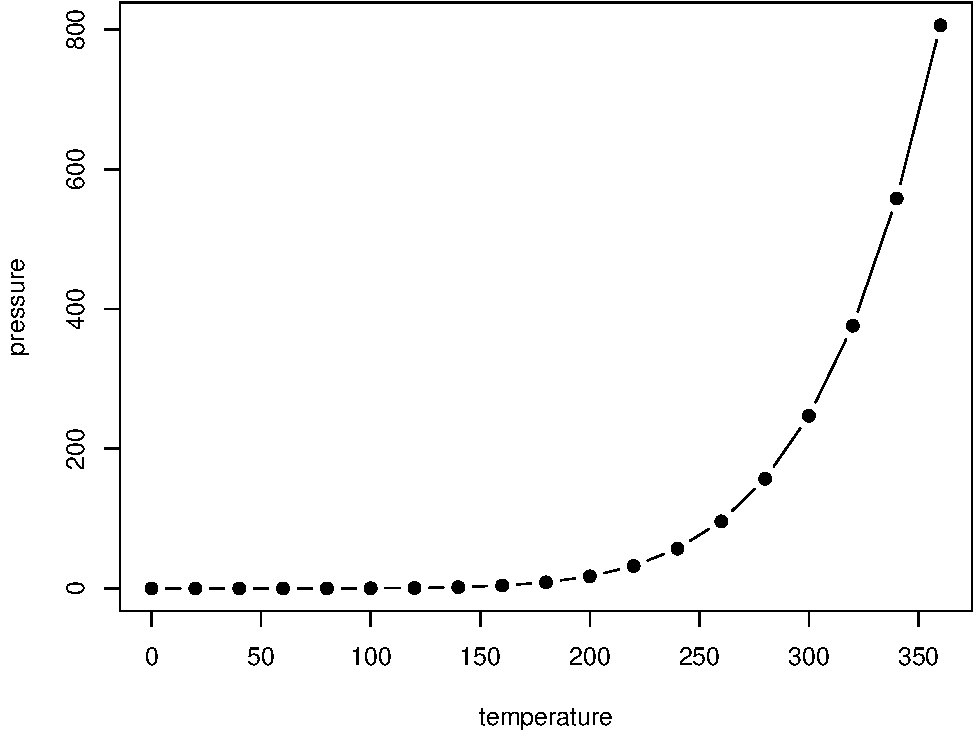
\includegraphics[width=0.8\linewidth]{predissertation_files/figure-latex/nice-fig-1} 

}

\caption{Here is a nice figure!}\label{fig:nice-fig}
\end{figure}

Reference a figure by its code chunk label with the \texttt{fig:}
prefix, e.g., see Figure \ref{fig:nice-fig}.

\hypertarget{tables}{%
\section{Tables}\label{tables}}

The easiest way to create a table is to use Excel to input the
information for your table and save it as a CSV file. Then you can read
in the CSV file, and use the \texttt{kable()} function from
\textbf{knitr} to style the table.

\begin{Shaded}
\begin{Highlighting}[]
\CommentTok{#Read in data}
\NormalTok{gopher =}\StringTok{ }\NormalTok{readr}\OperatorTok{::}\KeywordTok{read_csv}\NormalTok{(}\StringTok{"data/tab-gopher-women-sports.csv"}\NormalTok{)}
\end{Highlighting}
\end{Shaded}

\begin{verbatim}
## Parsed with column specification:
## cols(
##   Sport = col_character(),
##   `Ticket Sales` = col_integer(),
##   `Total Operating Revenue` = col_integer()
## )
\end{verbatim}

\begin{Shaded}
\begin{Highlighting}[]
\CommentTok{# Create table}
\NormalTok{knitr}\OperatorTok{::}\KeywordTok{kable}\NormalTok{(}
\NormalTok{  gopher, }
  \DataTypeTok{caption =} \StringTok{"2017 Ticket Sales and Operating Revenue for the University of Minnesota Women's Athletic Teams"}\NormalTok{,}
  \DataTypeTok{booktabs =} \OtherTok{TRUE}
\NormalTok{)}
\end{Highlighting}
\end{Shaded}

\begin{table}

\caption{\label{tab:nice-tab}2017 Ticket Sales and Operating Revenue for the University of Minnesota Women's Athletic Teams}
\centering
\begin{tabular}[t]{lrr}
\toprule
Sport & Ticket Sales & Total Operating Revenue\\
\midrule
Basketball & 252009 & 873843\\
Cross Country &  & \\
Golf &  & 45197\\
Gymnastics & 38287 & 58288\\
Hockey & 110926 & 389769\\
\addlinespace
Rowing &  & 45454\\
Soccer & 14868 & 33374\\
Softball & 42074 & 98003\\
Swimming \& Diving &  & 74894\\
Tennis &  & 11392\\
\addlinespace
Track and Field &  & 24101\\
Volleyball & 337492 & 485157\\
\bottomrule
\end{tabular}
\end{table}

Further table styling can be carried out via the \textbf{kableExtra}
package; see
\url{https://haozhu233.github.io/kableExtra/awesome_table_in_pdf.pdf}.
Below we demonstrate some of that functionality.

\begin{Shaded}
\begin{Highlighting}[]
\KeywordTok{library}\NormalTok{(kableExtra)}

\NormalTok{knitr}\OperatorTok{::}\KeywordTok{kable}\NormalTok{(}
\NormalTok{  gopher, }
  \DataTypeTok{caption =} \StringTok{"2017 Ticket Sales and Operating Revenue for the University of Minnesota Women's Athletic Teams"}\NormalTok{,}
  \DataTypeTok{booktabs =} \OtherTok{TRUE}\NormalTok{,}
  \DataTypeTok{format =} \StringTok{"latex"}
\NormalTok{  ) }\OperatorTok
\StringTok{  }\KeywordTok{footnote}\NormalTok{(}\DataTypeTok{general =} \StringTok{"Data obtained from the 2017 NCAA Financial Report"}\NormalTok{)}
\end{Highlighting}
\end{Shaded}

\begin{table}

\caption{\label{tab:nice-tab-2}2017 Ticket Sales and Operating Revenue for the University of Minnesota Women's Athletic Teams}
\centering
\begin{tabular}[t]{lrr}
\toprule
Sport & Ticket Sales & Total Operating Revenue\\
\midrule
Basketball & 252009 & 873843\\
Cross Country &  & \\
Golf &  & 45197\\
Gymnastics & 38287 & 58288\\
Hockey & 110926 & 389769\\
\addlinespace
Rowing &  & 45454\\
Soccer & 14868 & 33374\\
Softball & 42074 & 98003\\
Swimming \& Diving &  & 74894\\
Tennis &  & 11392\\
\addlinespace
Track and Field &  & 24101\\
Volleyball & 337492 & 485157\\
\bottomrule
\multicolumn{3}{l}{\textbf{Note: } }\\
\multicolumn{3}{l}{Data obtained from the 2017 NCAA Financial Report}\\
\end{tabular}
\end{table}

You can also create the table from within R itself and then use
\texttt{kable()}.

\begin{Shaded}
\begin{Highlighting}[]
\NormalTok{tab =}\StringTok{ }\NormalTok{flights }\OperatorTok
\StringTok{  }\KeywordTok{filter}\NormalTok{(month }\OperatorTok{==}\StringTok{ }\DecValTok{12}\NormalTok{, day }\OperatorTok{==}\StringTok{ }\DecValTok{24}\NormalTok{) }\OperatorTok
\StringTok{  }\KeywordTok{group_by}\NormalTok{(carrier_name) }\OperatorTok
\StringTok{  }\KeywordTok{summarize}\NormalTok{(}
    \DataTypeTok{Departure =} \KeywordTok{mean}\NormalTok{(dep_delay),}
    \DataTypeTok{Arrival =} \KeywordTok{mean}\NormalTok{(arr_delay)}
\NormalTok{    ) }\OperatorTok
\StringTok{  }\KeywordTok{select}\NormalTok{(}\DataTypeTok{Carrier =}\NormalTok{ carrier_name, Departure, Arrival)}

\NormalTok{knitr}\OperatorTok{::}\KeywordTok{kable}\NormalTok{(}
\NormalTok{  tab, }
  \DataTypeTok{caption =} \StringTok{"Average Departure and Arrival Delay (in Minutes) by Carrier on Decemebr 24"}\NormalTok{,}
  \DataTypeTok{booktabs =} \OtherTok{TRUE}\NormalTok{,}
  \DataTypeTok{format =} \StringTok{"latex"}\NormalTok{,}
  \DataTypeTok{digits =} \DecValTok{2}
\NormalTok{  )}
\end{Highlighting}
\end{Shaded}

\begin{table}

\caption{\label{tab:unnamed-chunk-3}Average Departure and Arrival Delay (in Minutes) by Carrier on Decemebr 24}
\centering
\begin{tabular}[t]{lrr}
\toprule
Carrier & Departure & Arrival\\
\midrule
Alaska Airlines Inc. & -2.65 & -0.39\\
American Airlines Inc. & -6.25 & -18.75\\
Delta Air Lines Inc. & -0.36 & -4.55\\
Frontier Airlines Inc. & -9.67 & -20.33\\
Hawaiian Airlines Inc. & -2.00 & 22.00\\
\addlinespace
JetBlue Airways & -6.67 & -14.33\\
SkyWest Airlines Inc. & -6.43 & -10.86\\
Southwest Airlines Co. & 16.83 & 9.04\\
United Air Lines Inc. & 9.55 & 3.00\\
US Airways Inc. & -2.17 & -0.50\\
Virgin America & -2.00 & 4.00\\
\bottomrule
\end{tabular}
\end{table}

You can also reference tables generated from \texttt{knitr::kable()},
e.g., see Table \ref{tab:nice-tab}.

\hypertarget{results}{%
\chapter{Results}\label{results}}

This chapter includes your analyses and results. It should include:

\begin{itemize}
\tightlist
\item
  General data analysis and results
\item
  Data results specific to each hypothesis are presented
\item
  Chapter review
\end{itemize}

\hypertarget{figures-1}{%
\section{Figures}\label{figures-1}}

If your thesis has a lot of figures, \emph{R Markdown} might behave
better for you than that other word processor. One perk is that it will
automatically number the figures accordingly in each chapter. You'll
also be able to create a label for each figure, add a caption, and then
reference the figure in a way similar to what we saw with tables
earlier. If you label your figures, you can move the figures around and
\emph{R Markdown} will automatically adjust the numbering for you. No
need for you to remember! So that you don't have to get too far into
LaTeX to do this, a couple \textbf{R} functions have been created for
you to assist. You'll see their use below.

In the \textbf{R} chunk below, we will load in a picture stored as
\texttt{goldy.png} in our \texttt{figures} directory. We then give it
the caption of ``Goldy rendered as a pencil drawing.'', the label of
``goldy'', and specify that this is a figure. Make note of the different
\textbf{R} chunk options that are given in the R Markdown file (not
shown in the knitted document).

\begin{Shaded}
\begin{Highlighting}[]
\KeywordTok{include_graphics}\NormalTok{(}\DataTypeTok{path =} \StringTok{"figures/goldy.png"}\NormalTok{)}
\end{Highlighting}
\end{Shaded}

\begin{figure}

\includegraphics[width=1.39in]{figures/goldy} \caption{Goldy rendered as a pencil drawing.}\label{fig:goldy}
\end{figure}

Here is a reference to the Goldy image: Figure \ref{fig:goldy}. Note the
use of the \texttt{fig:} code here. By naming the \textbf{R} chunk that
contains the figure, we can then reference that figure later as done in
the first sentence here. We can also specify the caption for the figure
via the R chunk option \texttt{fig.cap}.

Notice the figure was floated to the top of the page. To override this,
we use the chunk option \texttt{pos="H"}. That will override the float
and place the figure exactly where the code chunk is.

\begin{Shaded}
\begin{Highlighting}[]
\KeywordTok{include_graphics}\NormalTok{(}\DataTypeTok{path =} \StringTok{"figures/goldy.png"}\NormalTok{)}
\end{Highlighting}
\end{Shaded}

\begin{figure}[H]

\includegraphics[width=1.39in]{figures/goldy} \caption{Goldy still rendered as a pencil drawing. This time we overrode the float using the 'H' option.}\label{fig:goldy2}
\end{figure}

Below we will investigate how to save the output of an \textbf{R} plot
and label it in a way similar to that done above. Recall the
\texttt{flights} dataset from Chapter \ref{rmd-basics}. (Note that we've
shown a different way to reference a section or chapter here.) We will
next explore a bar graph with the mean flight departure delays by
airline from Portland for 2014. Note also the use of the \texttt{scale}
parameter which is discussed on the next page.

\begin{Shaded}
\begin{Highlighting}[]
\NormalTok{flights }\OperatorTok\StringTok{ }\KeywordTok{group_by}\NormalTok{(carrier) }\OperatorTok
\StringTok{ }\KeywordTok{summarize}\NormalTok{(}\DataTypeTok{mean_dep_delay =} \KeywordTok{mean}\NormalTok{(dep_delay)) }\OperatorTok
\StringTok{ }\KeywordTok{ggplot}\NormalTok{(}\KeywordTok{aes}\NormalTok{(}\DataTypeTok{x =}\NormalTok{ carrier, }\DataTypeTok{y =}\NormalTok{ mean_dep_delay)) }\OperatorTok{+}
\StringTok{ }\KeywordTok{geom_bar}\NormalTok{(}\DataTypeTok{position =} \StringTok{"identity"}\NormalTok{, }\DataTypeTok{stat =} \StringTok{"identity"}\NormalTok{, }\DataTypeTok{fill =} \StringTok{"red"}\NormalTok{)}
\end{Highlighting}
\end{Shaded}

\begin{figure}
\centering
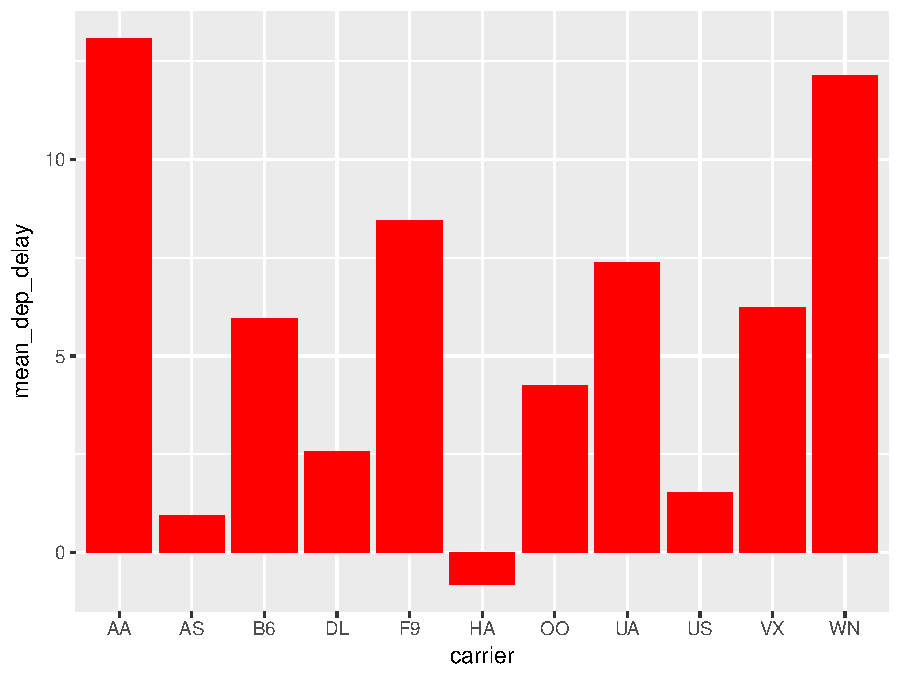
\includegraphics{predissertation_files/figure-latex/delaysboxplot-1.pdf}
\caption{\label{fig:delaysboxplot}Mean Delays by Airline}
\end{figure}

Here is a reference to this image: Figure \ref{fig:delaysboxplot}.

\clearpage

\hypertarget{citations}{%
\section{Citations}\label{citations}}

You can write citations, too. For example, we are using the
\textbf{bookdown} package \citep{R-bookdown} in this sample book, which
was built on top of R Markdown and \textbf{knitr} \citep{xie2015}.

\hypertarget{footnotes-and-endnotes}{%
\section{Footnotes and Endnotes}\label{footnotes-and-endnotes}}

You might want to footnote something. \footnote{footnote text} The
footnote will be in a smaller font and placed appropriately. Endnotes
work in much the same way.

\hypertarget{bibliographies}{%
\section{Bibliographies}\label{bibliographies}}

Of course you will need to cite things, and you will probably accumulate
an armful of sources. There are a variety of tools available for
creating a bibliography database (stored with the .bib extension). In
addition to BibTeX suggested below, you may want to consider using the
free and easy-to-use tool called Zotero. Some Zotero documentation is at
\url{http://libguides.reed.edu/citation/zotero}. In addition, a tutorial
is available from Middlebury College at
\url{http://sites.middlebury.edu/zoteromiddlebury/}.

\emph{R Markdown} uses \emph{pandoc} (\url{http://pandoc.org/}) to build
its bibliographies. One nice caveat of this is that you won't have to do
a second compile to load in references as standard LaTeX requires. To
cite references in your thesis (after creating your bibliography
database), place the reference name inside square brackets and precede
it by the ``at'' symbol. For example, here's a reference to a book about
worrying: \citep{Molina1994}. This \texttt{Molina1994} entry appears in
a file called \texttt{thesis.bib} in the \texttt{bib} folder. This
bibliography database file was created by a program called BibTeX. You
can call this file something else if you like (look at the YAML header
in the main .Rmd file) and, by default, is to placed in the \texttt{bib}
folder.

For more information about BibTeX and bibliographies, see
(\url{http://web.reed.edu/cis/help/latex/index.html})\footnote{\citet{reedweb2007}}.
There are three pages on this topic: \emph{bibtex} (which talks about
using BibTeX, at \url{http://web.reed.edu/cis/help/latex/bibtex.html}),
\emph{bibtexstyles} (about how to find and use the bibliography style
that best suits your needs, at
\url{http://web.reed.edu/cis/help/latex/bibtexstyles.html}) and
\emph{bibman} (which covers how to make and maintain a bibliography by
hand, without BibTeX, at
\url{http://web.reed.edu/cis/help/latex/bibman.html}). The last page
will not be useful unless you have only a few sources.

If you look at the YAML header at the top of the main .Rmd file you can
see that we can specify the style of the bibliography by referencing the
appropriate csl file. You can download a variety of different style
files at \url{https://www.zotero.org/styles}. Make sure to download the
file into the csl folder.

\textbf{Tips for Bibliographies}

\begin{itemize}
\tightlist
\item
  Like with thesis formatting, the sooner you start compiling your
  bibliography for something as large as thesis, the better.
\item
  The cite key (a citation's label) needs to be unique from the other
  entries.
\item
  When you have more than one author or editor, you need to separate
  each author's name by the word ``and'' e.g.
  \texttt{Author\ =\ \{Noble,\ Sam\ and\ Youngberg,\ Jessica\},}.
\item
  Bibliographies made using BibTeX (whether manually or using a manager)
  accept LaTeX markup, so you can italicize and add symbols as
  necessary.
\item
  To force capitalization in an article title or where all lowercase is
  generally used, bracket the capital letter in curly braces.
\end{itemize}

\hypertarget{discussion}{%
\chapter{Discussion}\label{discussion}}

Summarize the entire project including what hypothesis/questions were
investigated, why they were investigated, how they were investigated,
the major findings, and your conclusions.

\begin{enumerate}
\def\labelenumi{\arabic{enumi}.}
\tightlist
\item
  Discuss the findings and the hypothesis in a holistic and integrated
  fashion.
\item
  Explain any extraneous factors that may have led to the results you
  obtained.
\item
  Discuss the practical and theoretical implications of your findings
  and precisely how your research supports each implication.
\item
  State the conclusions to be drawn from your entire study (including
  review of the literature and empirical findings; i.e., integrate
  everything).
\item
  Discuss suggestion for future research, next stages of research, what
  others might do to follow up on your study.
\end{enumerate}

\hypertarget{anything-else}{%
\section{Anything else?}\label{anything-else}}

If you would like to see examples of other things in this template,
please contact me at \url{zief0002@umn.edu} with your suggestions. I
love to see people using \emph{R Markdown} for their theses, and am
happy to help.

\bibliography{bib/book.bib,bib/packages.bib}


\end{document}
